%%%%%%%%%%%%%%%%%%%%%%%%%%%%%%%%%%%%%%%%%%%%%%%%%%%%%%%%%%%%
% Dokument-Einstellungen
\documentclass{SMBV12}

\setcounter{tocdepth}{5} %to make it appears in TOC
\setcounter{secnumdepth}{5} %to make it numbered

%%%%%%%%%%%%%%%%%%%%%%%%%%%%%%%%%%%%%%%%%%%%%%%%%%%%%%%%%%%%
%-----------------------------------------------------------
% Hier beginnt das eigentliche Dokument
\begin{document}

\title{Graph-Based Segmentation}

\author{Phan-Anh Nguyen}

\maketitle

%%%%%%%%%%%%%%%%%%%%%%%%%%%%%%%%%%%%%%%%%%%%%%%%%%%%%%%%%%%%
%-----------------------------------------------------------% Zusammenfassung

\begin{abstract}%
Abstract. This 20-page seminar paper reviews the state-of-the-art graph-based segmentation algorithms.
\end{abstract}

\keywords{Classification, Graph Cut, Segmentation}


%%%%%%%%%%%%%%%%%%%%%%%%%%%%%%%%%%%%%%%%%%%%%%%%%%%%%%%%%%%%
%-----------------------------------------------------------
%
\section{Introduction}

Introduction is written at last.

%%%%%%%%%%%%%%%%%%%%%%%%%%%%%%%%%%%%%%%%%%%%%%%%%%%%%%%%%%%%
%-----------------------------------------------------------
%
\section{Image Features}

%%%%%%%%%%%%%%%%%%%%%%%%%%%%%%%%%%%%%%%%%%%%%%%%%%%%%%%%%%%%
\subsection{Image Feature Overview}
%What are image features? How can we describe/represent them?
Low level image features are essential building blocks for high level image processing tasks such as object detection, image categorization or segmentation etc. In general, image features capture important properties around local image regions in the form of high dimensional feature vectors that can be used by high level applications. Normally, raw features are extracted at each pixel by applying various kinds of filters. Each filter response contributes one dimension in the feature vector space. The shape and size of filters reflect local structure around each pixel. Raw features at each pixel can be collected to form region descriptors which can be used to represent shapes, contours etc. In this section we present methods to extract raw features and various ways of constructing region descriptors. Specifically, Section $\ref{sec:surf}$ describes a state-of-the-art feature named SURF (Speeded Up Robust Features) \cite{bay2006surf} and Section $\ref{sec:shape_feature}$ explains the gPb (globalized probability of boundary) contour extractor \cite{maire2008using}.


%%%%%%%%%%%%%%%%%%%%%%%%%%%%%%%%%%%%%%%%%%%%%%%%%%%%%%%%%%%%
\subsection{SURF Feature}
\label{sec:surf}
SURF \cite{bay2006surf} was originally developed for the task of finding point correspondences between two images of the same scene. This includes three main steps. First, "interest points" are
selected at distinctive locations in the image. Then a feature vector is extracted from the neighbourhood of every interest point. Finally the feature vectors are matched between different images. Since the SURF descriptor provides a very good representation of a local region it has been applied to other tasks such as image classification or image segmentation.

Regarding the interest point detection problem, the choice of the detector varies depending on the application need. In an image registration application, it is required that the same interest points be detected in two different images of the same scene under different viewing conditions. In this case, the good detector would pick up corner points. In the case of image segmentation, it would be a wise choice to select points on contours to be interest points. In the original SURF paper, Bay et al. suggested using approximate Hessian detector to search in scale-space domain for points having strong derivatives in two orthogonal directions as interest points (often located at corners and strongly textured areas).

Given an interest point in the input image, the SURF descriptor is obtained by extracting distinctive information around its neighbourhood in a form of a feature vector. The SURF descriptor is designed to be invariant to image scaling and rotation while it has to be computed very fast. Scale invariance is achieved by adopting the scale at which the Hessian detector attains maximal response. In order to be invariant to rotation, we first find a reproducible orientation based on information within a circular region around the interest point. We then construct a square region aligned to the selected orientation and extract the SURF descriptor from it.

To find the dominant orientation, the Haar wavelet responses in $x$ and $y$ directions, ($d_x$, $d_y$), are calculated within a circular neighbourhood of radius $6s$ around the interest point and weighted with a Gaussian ($\sigma = 2s$), where $s$ is the scale chosen above. Figure $\ref{fig:haar_wavelet}$ shows the structure of the Haar wavelet filters. The wavelet responses ($d_x, d_y$) are then represented in a vector space and the sum of all vectors within a sliding orientation window of size $\pi/3$ are calculated, see Figure $\ref{fig:orientation_window}$. The dominant orientation is finally assigned to the sum vector having the maximal length.

\begin{figure}[htbp]
    \centering
    \subfigure[]
    {
        
\includegraphics[width=0.15\textwidth]{images/haar_wavelet.png}
        \label{fig:haar_wavelet}
    }
    \subfigure[]
    {
        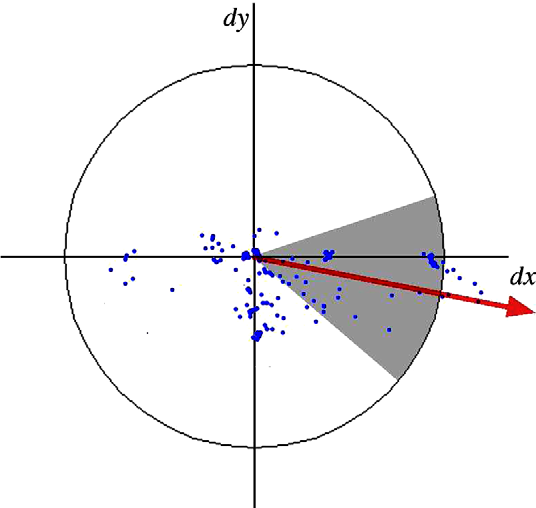
\includegraphics[width=0.25\textwidth]{images/orientation_window.png}
        \label{fig:orientation_window}
    }
    \subfigure[]
    {
        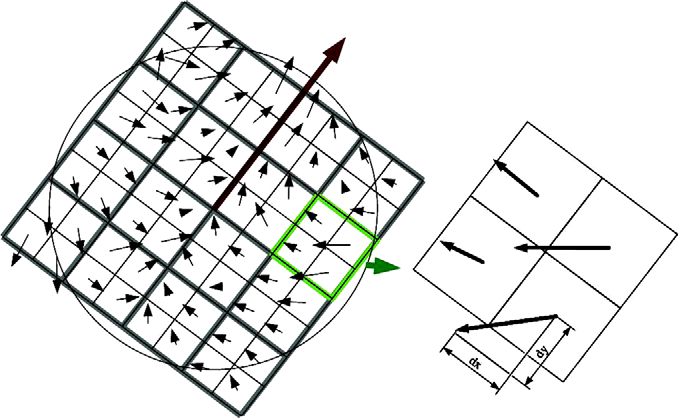
\includegraphics[width=0.5\textwidth]{images/surf.png}
        \label{fig:surf}
    }
    \caption{(a) Haar wavelet filters for the x (left) and y (right) components. The dark parts are weighted -1 and the light parts +1. (b) Orientation assignment: a sliding orientation window of size $\pi/3$ detects the dominant orientation. (c) The SURF descriptor: an oriented quadratic grid with $4 \times 4$ square cells is laid over the interest point (left). For each cell, the wavelet responses are computed from $5 \times 5$ samples (for illustrative
    purposes, only $2 \times 2$ sub-divisions are shown here). In each cell, the 4 elements $\sum d_x$, $\sum \left| d_x \right|$, $\sum d_y$, $\sum \left| d_y \right| $ contribute to the SURF feature vector. } 
    %\label{fig:surf}
\end{figure}

To extract the SURF descriptor, we construct a window of size $20s$ centred at the interest point and oriented in the dominant orientation as illustrated in Figure $\ref{fig:surf}$. The window is then subdivided into a regular $4 \times 4$ grid cells, each being a $5 \times 5$ pixel patch. For each cell, the Gaussian weighted ($\sigma = 3.3s$) Haar wavelet responses are summed up to form a first set of entries in the feature vector. The sum of the absolute values of the responses, $\left| d_x \right| $ and $\left| d_y \right| $ are also extracted to capture information about the polarity of the intensity changes. Therefore, each cell has a 4D descriptor vector for its underlying intensity structure $\left( \sum d_x, \sum d_y, \sum \left| d_x \right| , \sum \left| d_y \right|  \right)$. Concatenating this for all $4 \times 4$ cells results in a descriptor vector of length 64. Finally the descriptor vector is normalized to make it invariant to contrast.

%%%%%%%%%%%%%%%%%%%%%%%%%%%%%%%%%%%%%%%%%%%%%%%%%%%%%%%%%%%%
\subsection{gPb Contour Extractor}
\label{sec:shape_feature}

introduction to gPb

\subsubsection{Gradient-Based Features}

The gradient-based paradigm was used by Martin et al. in their $Pb$ paper \cite{martin2004learning} to detect local changes in color, texture and brightness. Basically at each pixel location $(x, y)$, a circle of radius $r$ is drawn and cut half along the diameter having orientation $\theta$. The gradient function $G(x, y, \theta, r)$ is used to compare the contents of the two resulting half disks. An edge is detected if there is a large difference between the two half disks along the chosen orientation.

To represent the color and brightness contents within a half disk, histograms are built by sampling the Gaussian kernel density estimates of brightness and color in CIELAB color space. The L* channel is used to compute brightness histogram and the a* and b* are used to compute color histogram. The bin size is chosen such that each bin contains at least 2 Gaussian kernels of size $2\sigma$. Figure $\ref{fig:kde}$ shows an example of a Gaussian kernel density estimate. The $\chi^2$ distance is used to compute the difference between histograms:
\begin{equation}
	\chi^2(g, h) = 1/2\sum \dfrac{(g_i - h_i)^2}{g_i + h_i}
\end{equation}

\begin{figure}[htbp]
    \centering
    \subfigure[]
    {
        \includegraphics[width=0.2\textwidth]{images/kde.png}
        \label{fig:kde}
    }
    \subfigure[]
    {
        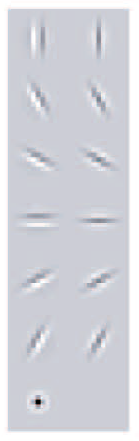
\includegraphics[width=0.1\textwidth]{images/filter_bank.png}
        \label{fig:filter_bank}
    }
    \subfigure[]
    {
        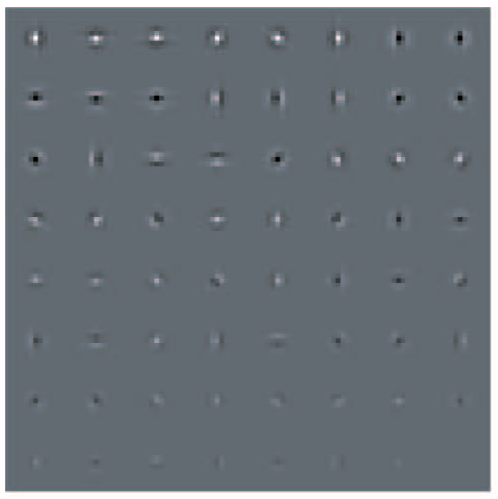
\includegraphics[width=0.2\textwidth]{images/textons.png}
        \label{fig:textons}
    }
    \subfigure[]
    {
        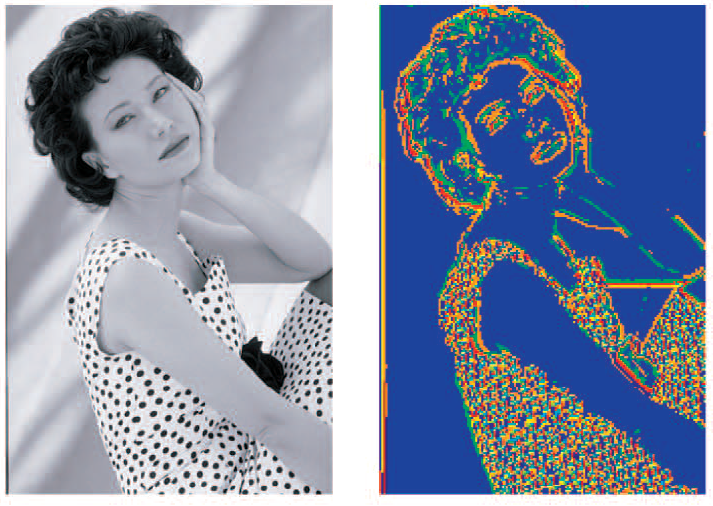
\includegraphics[width=0.4\textwidth]{images/texture_map.png}
        \label{fig:texture_map}
    }
    \caption{  } 
    %\label{fig:texture}
\end{figure}

Considering the problem of computing texture gradient, a group of 13 filters covering the most probable shapes is used. Particularly, it consists of six pairs of elongated, oriented filters and a center-surround filter as shown in Figure $\ref{fig:filter_bank}$. The oriented filters are in even/odd quadrature pairs. The even symmetric filter is a Gaussian second derivative, and the odd-symmetric filter is its Hilbert transform. Finally, a difference of Gaussians is chosen to be the center-surround filter. This filter bank generates a feature vector of 13 dimensions corresponding to 13 filter responses at each pixel.

In order to build up histograms for comparison, the $Pb$ algorithm uses the so called textons approach (or bag of textures approach) introduced by Malik et al. \cite{malik2001contour}. The basic idea is to cluster the filter response vectors over a large, diverse collection of training images using k-means. Each cluster defines a Voronoi cell in the space of joint filter responses, and the cluster centers, textons, represent texture primitives. Figure $\ref{fig:textons}$ illustrates example textons for k = 64 computed over the 200 images in the training set. Once the dictionary of textons have been computed, each pixel is assigned to the nearest texton. Figure $\ref{fig:texture_map}$ shows an image and the associated texton map, where each pixel has been labeled with the nearest texton. Finally the histograms of activated textons in the two disc halves can be computed and compared using the $\chi^2$ distance operator.

\subsubsection{gPb Feature}

The gPb contour detector \cite{maire2008using} is an extension of Pb contour detector into which global information is integrated via spectral graph theory. Particularly, the gPb algorithm follows the idea of the normalized cut algorithm which defines an affinity matrix $W$ whose entries encode the similarity between pixels. The generalized eigenvectors of the following linear system provide global segmentation information:
\begin{equation}
(D-W)\mathbf{v} = \lambda D \mathbf{v}
\label{eq:ncut}
\end{equation}
where $D$ is diagonal matrix with $D_{ii} = \sum_j W_{ij}$.
Section $\ref{sec:normalized_cut}$ will explain the normalized cut algorithm in more detail.

We start by extracting the brightness, color and texture gradients in 3 different scales: $[\sigma/2, \sigma, 2\sigma]$, where $\sigma$ is the default scale of the Pb detector. This gives 9 different responses ${G_i}$. These local cues are then linearly combined into a single multiscale oriented signal:

\begin{equation}
mPb(x, y, \theta) = \sum\limits_{i = 1}^{9}G_i(x, y, \theta)
\end{equation}

In order to integrate global information, the affinity matrix $W$ is constructed by using the intervening contour cue \cite{leung1998contour}, that is, its entries are the maximal values of $mPb$ along a line connecting two pixels as shown in Figure $\ref{fig:intervening_contour}$. The first $k + 1$ generalized eigenvectors $\mathbf{v_j}$ of the system $\ref{eq:ncut}$ are chosen and reshaped in the size of the original image. Contours are extracted from each eigenvector $\mathbf{v_j}$ by applying Gaussian directional derivatives at multiple orientations $\theta$, resulting in an oriented signal $sPb_{\mathbf{v_j}}(x, y, \theta)$. The information from different eigenvectors is then combined to provide the "spectral" boundary detector:

\begin{equation}
sPb(x, y, \theta) = \sum\limits_{j=1}^{k}\dfrac{1}{\sqrt{\lambda_j}}sPb_{\mathbf{v_j}}(x, y, \theta)
\end{equation}

where $0 = \lambda_0 \leq ... \leq \lambda_k$ are corresponding eigenvalues. Figure $\ref{fig:sPb}$ illustrates an example of the spectral boundary detector $sPb$.

\begin{figure}[htbp]
    \centering
    \subfigure[]
    {
    	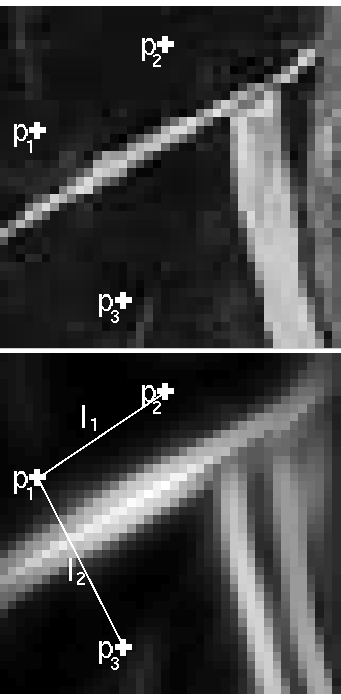
\includegraphics[width=0.15\textwidth]{images/intervening_contour.png}
        \label{fig:intervening_contour}
    }
    \subfigure[]
    {
    	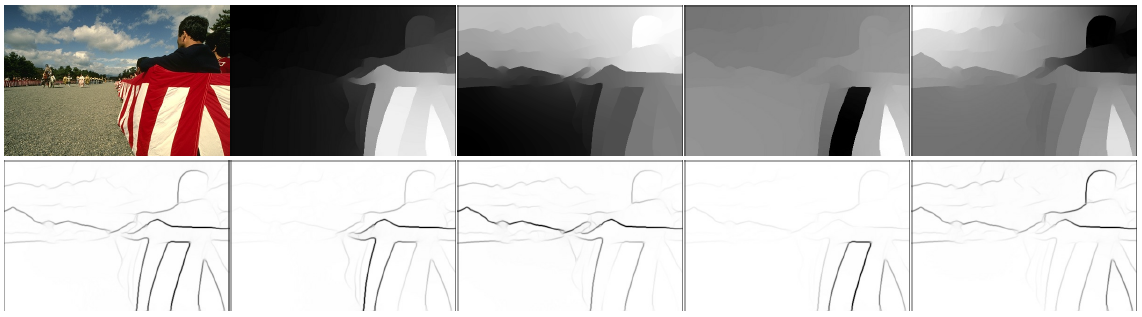
\includegraphics[width=0.8\textwidth]{images/sPb.png}
        \label{fig:sPb}
    }
    \caption{}
\end{figure}

Finally, the globalized probability of boundary , i.e. gPb, is then defined as:

\begin{equation}
gPb(x, y, \theta) = \sum\limits_{i = 1}^{9}\beta_i G_i(x, y, \theta) + \gamma sPb(x, y, \theta)
\end{equation}

where the weights are learned by gradient ascent on the F-measure = $2\cdot Precision \cdot Recall/(Precision + Recall)$.

\subsubsection{Shape Descriptor}

The contours detected above define over-segmented regions of the image. Gu et al. \cite{gu2009recognition} proposed a way to describe a region by subdividing evenly its bounding box into an $n \times n$ grid. The grid size n = 4 seems to be appropriate. Each cell encodes information only inside the region. Different cues are extracted from each cell, and each type of cue is encoded by concatenating cell signals into a histogram. The following region cues are included:

\begin{itemize}
\item Contour shape, given by the histogram of oriented responses of the contour detector gPb.
\item Edge shape, computed by convolution with a [-1 0 1] filter along x and y axes. This captures high frequency information, while it has been smoothed out by gPb.
\item Color, represented by the L*, a and b histograms in the CIELAB color space.
\item Texture, described by texton histograms.
\end{itemize}


%%%%%%%%%%%%%%%%%%%%%%%%%%%%%%%%%%%%%%%%%%%%%%%%%%%%%%%%%%%%
\subsection{Discussion}

pros and cons. Which descriptor is suitable for a particular case.

%\section{Supervised versus Unsupervised Segmentation Approaches}



\section{Supervised Learning Segmentation}

\subsection{Region Classification}

\subsubsection{Support Vector Machine}

\subsubsection{Structured SVM learning framework}

\cite{tsochantaridis2006large}

\subsection{Contour Classification}

\subsubsection{Logistic Regression}

\subsection{Statistical Shape Model}

\cite{leventon2000statistical}

%\subsection{Unsupervised Approaches}



\section{Graph Construction}

Intuitive connection between graphs and images.

\subsection{Region Graph}

\cite{arbelaez2009contours}

Vertex weight: point, shape features quantized by K-mean.
Edge weight: contour strength quantized by L-bin histogram and trained by the structured SVM learning framework.

Graph of small over-segmented regions. What is the advantage of this representation compared to branch and bound scheme. MWCS and PCST

\subsection{Contour Graph}

Circulation and Circle Embedding

\subsection{Markov Random Field}

\section{Graph Cut Algorithms}

comparison of cut algorithms, could them be used interchangeably in different situations.

\subsection{Prize-Collecting Steiner Tree}

\cite{ljubic2006algorithmic}

\subsubsection{Branch-and-Cut Algorithm}

\subsection{Hermitian Eigenvalue Problem}

\subsubsection{Normalized Cut}
\label{sec:normalized_cut}

\cite{shi2000normalized}

\subsubsection{Contour Cut}

\cite{zhu2007untangling}
\cite{KenGalShi2011}

\subsection{Graph-Cut}

\subsubsection{Min-Cut}

\subsubsection{Alpha-Expansion and Fusion Move}

\section{Applications}

System pipeline, result: accuracy, efficiency, benefits.

\subsection{Efficient Region Search for Object Detection}

\cite{VijayGrauman2011}

\subsection{Salient Contour Detection}

\cite{KenGalShi2011}

\subsection{Multi-Shape Graph-Cut for Lung Segmentation}

\cite{nakagomimulti}

\section{Conclusion}

lack of information: SURF at Canny points: what scale?
some criticisms e.g. time consuming, dataset used. Recommendation: what to use, why?

%%%%%%%%%%%%%%%%%%%%%%%%%%%%%%%%%%%%%%%%%%%%%%%%%%%%%%%%%%%%
%-----------------------------------------------------------
%
\def\refname{Literature}
%\begin{thebibliography}{AA}

\bibliographystyle{alpha}
\bibliography{bibliography}

%\end{thebibliography}

\newpage
\noindent
\begin{picture}(160,242)
\put(0,0){\framebox(160,242){}}
\end{picture}

\end{document}
